\section{Voraufgaben}

\subsection*{Aufgabe A}
\subsection*{Aufgabe B}
\subsection*{Aufgabe C}
% Theo
\begin{figure}[H]
    \centering
    \begin{subfigure}[b]{0.45\textwidth}
        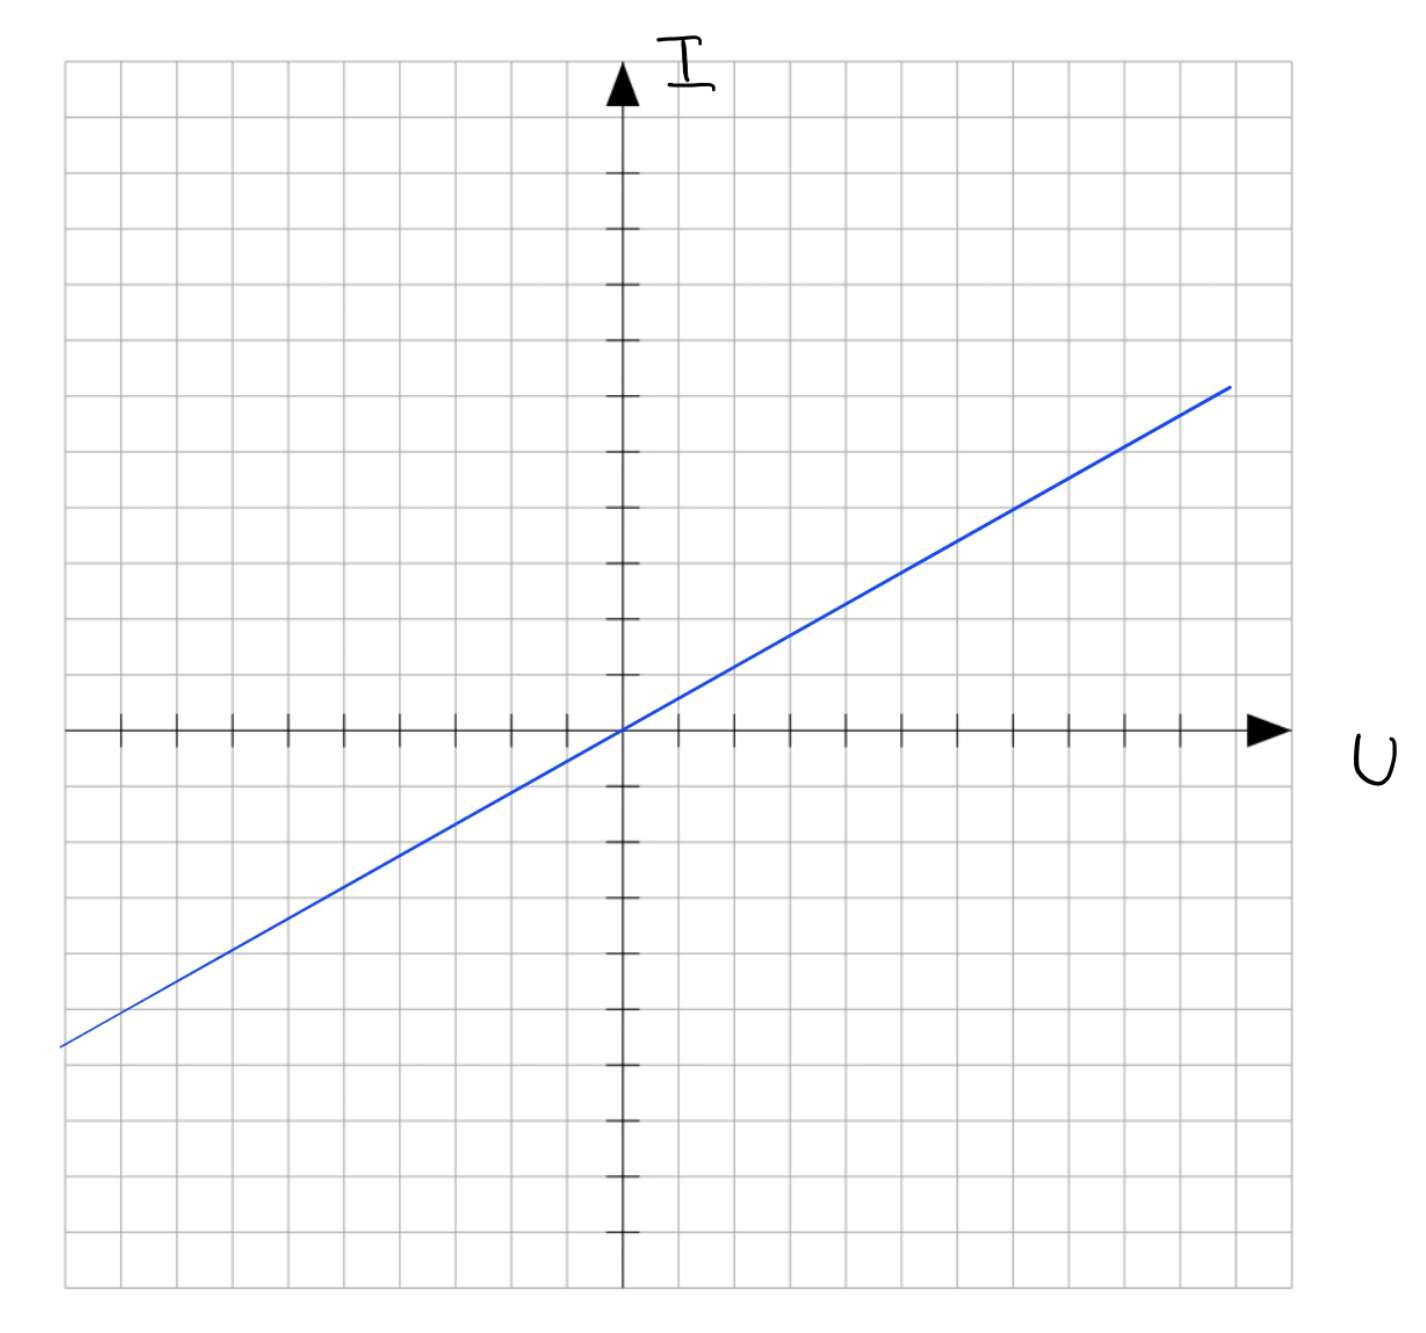
\includegraphics[width=\textwidth]{Voraufgaben/Ca.jpg}
        \caption{}
        \label{fig:VA_C_a}
    \end{subfigure}
    \hfill
    \begin{subfigure}[b]{0.45\textwidth}
        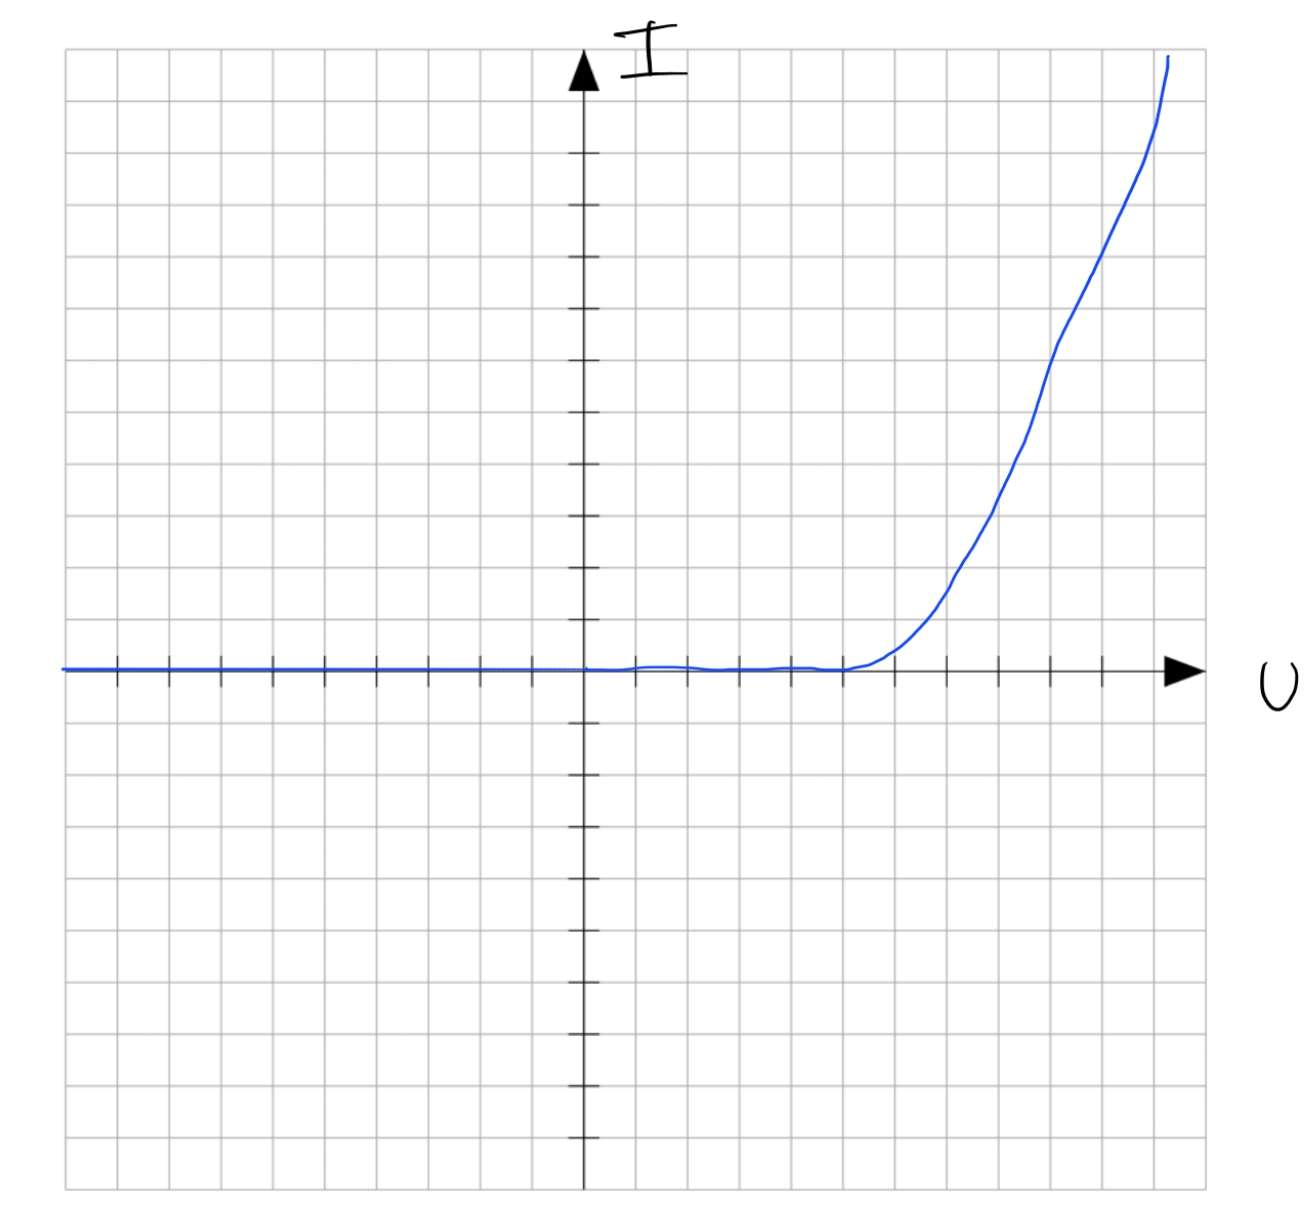
\includegraphics[width=\textwidth]{Voraufgaben/Cb.jpg}
        \caption{}
        \label{fig:VA_C_b}
    \end{subfigure}
    \vspace{0.5em}
    \begin{subfigure}[b]{0.45\textwidth}
        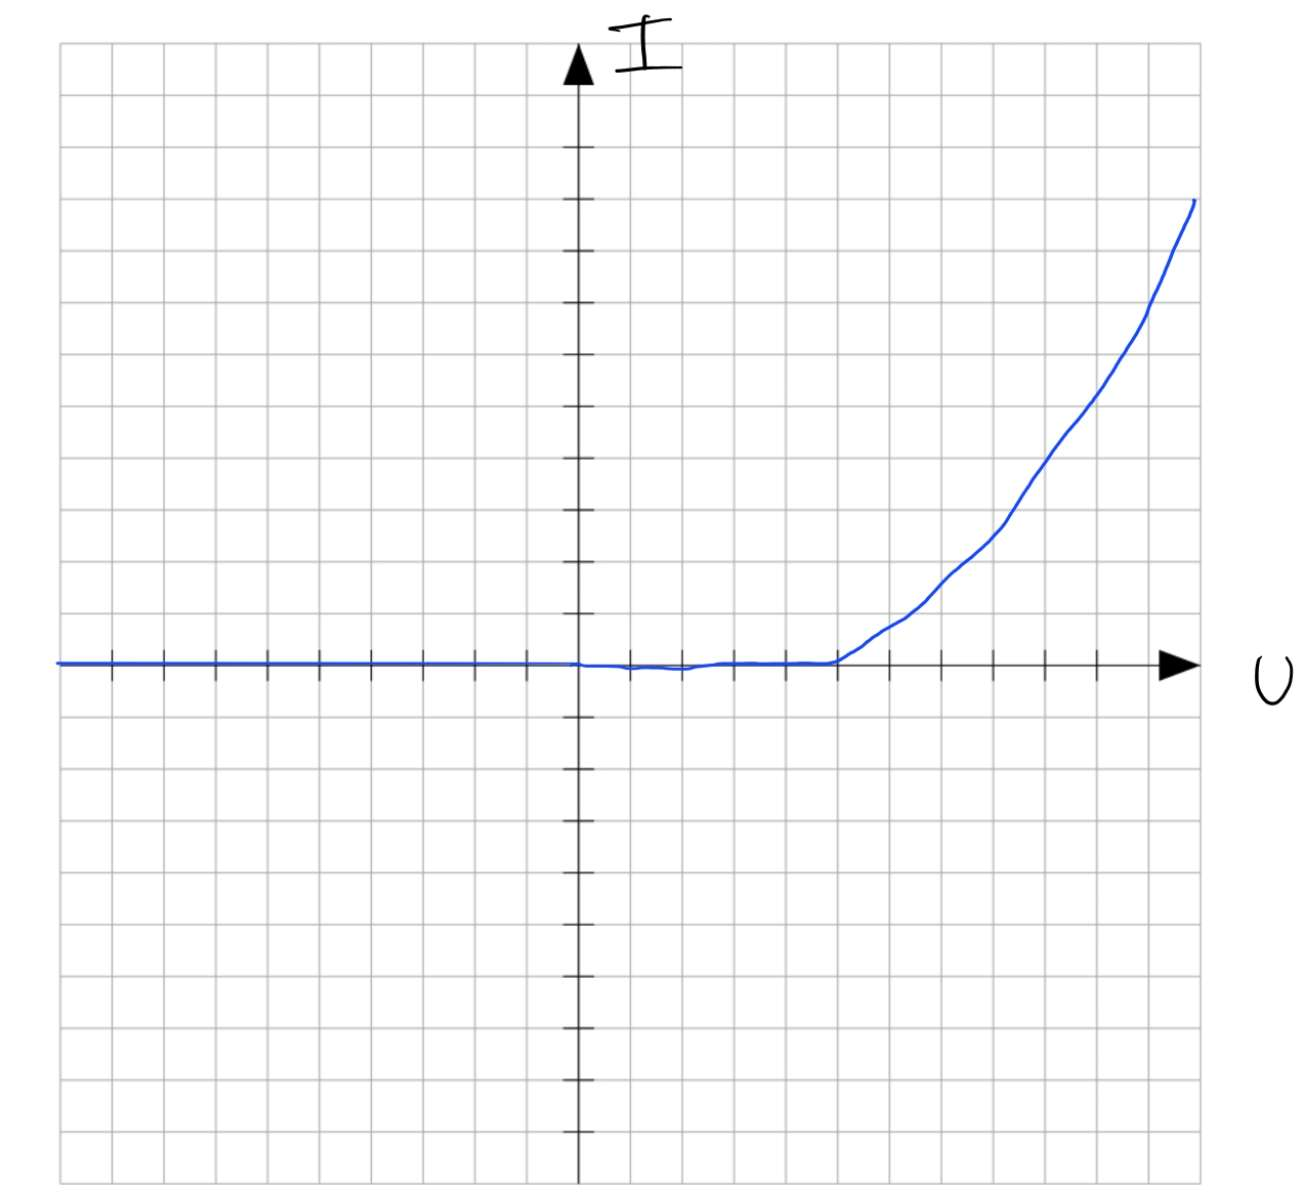
\includegraphics[width=\textwidth]{Voraufgaben/Cc.jpg}
        \caption{}
        \label{fig:VA_C_c}
    \end{subfigure}
    \hfill
    \begin{subfigure}[b]{0.45\textwidth}
        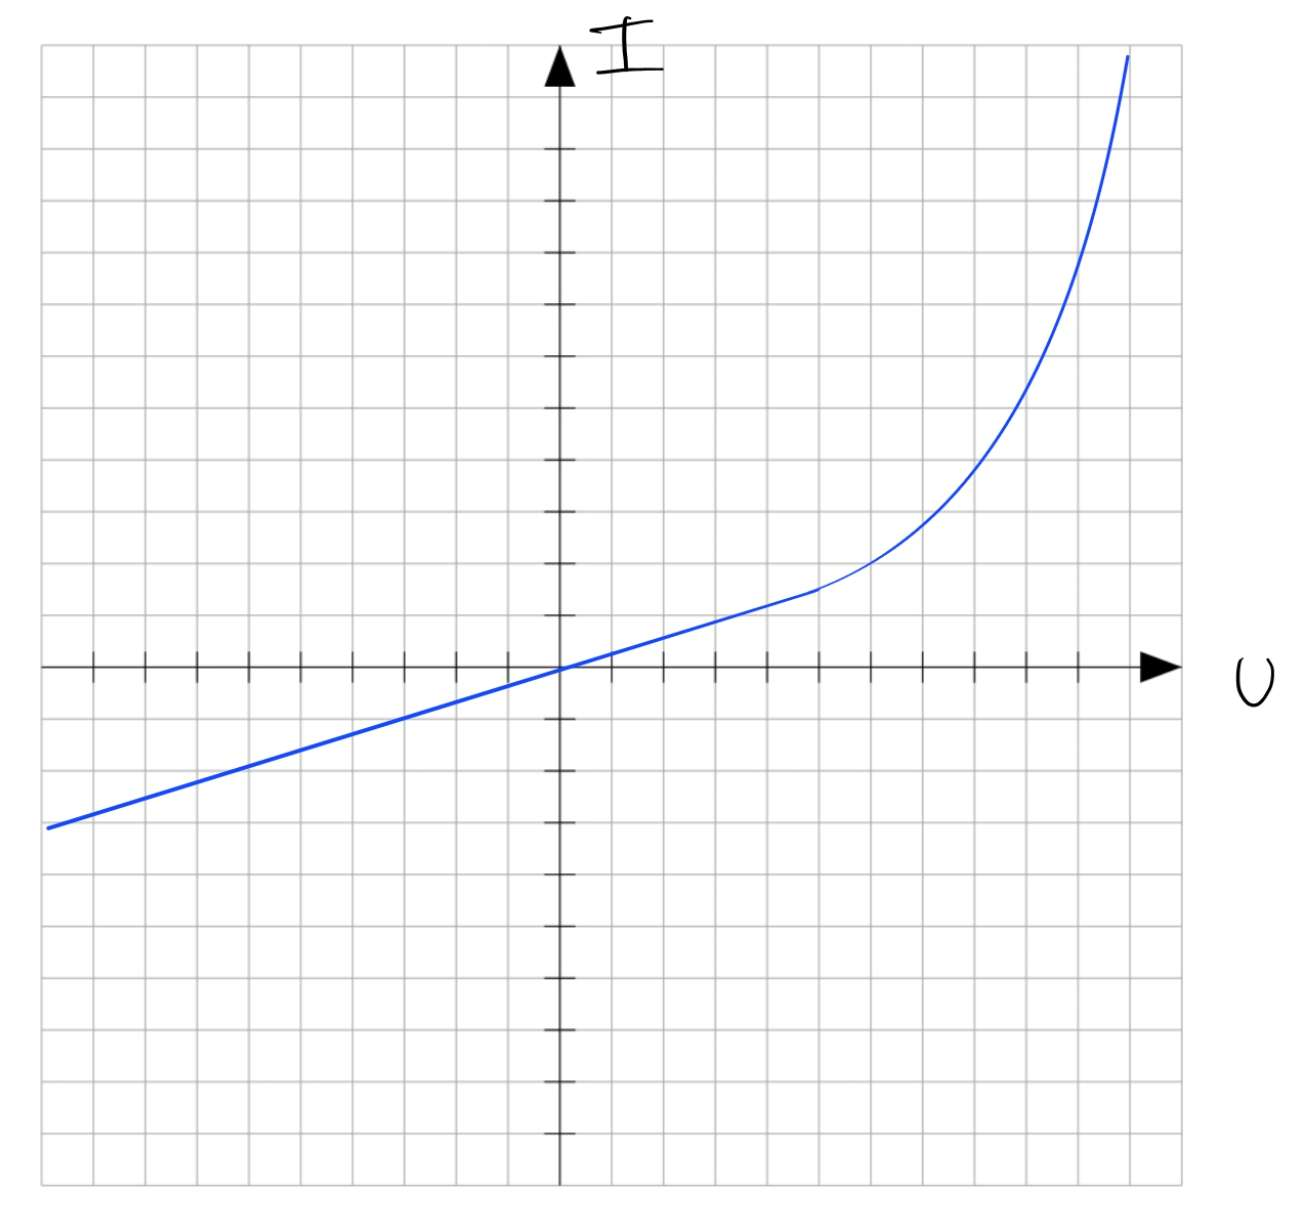
\includegraphics[width=\textwidth]{Voraufgaben/Cd.jpg}
        \caption{}
        \label{fig:VA_C_d}
    \end{subfigure}
    \vspace{0.5em}
    \begin{subfigure}[b]{0.45\textwidth}
        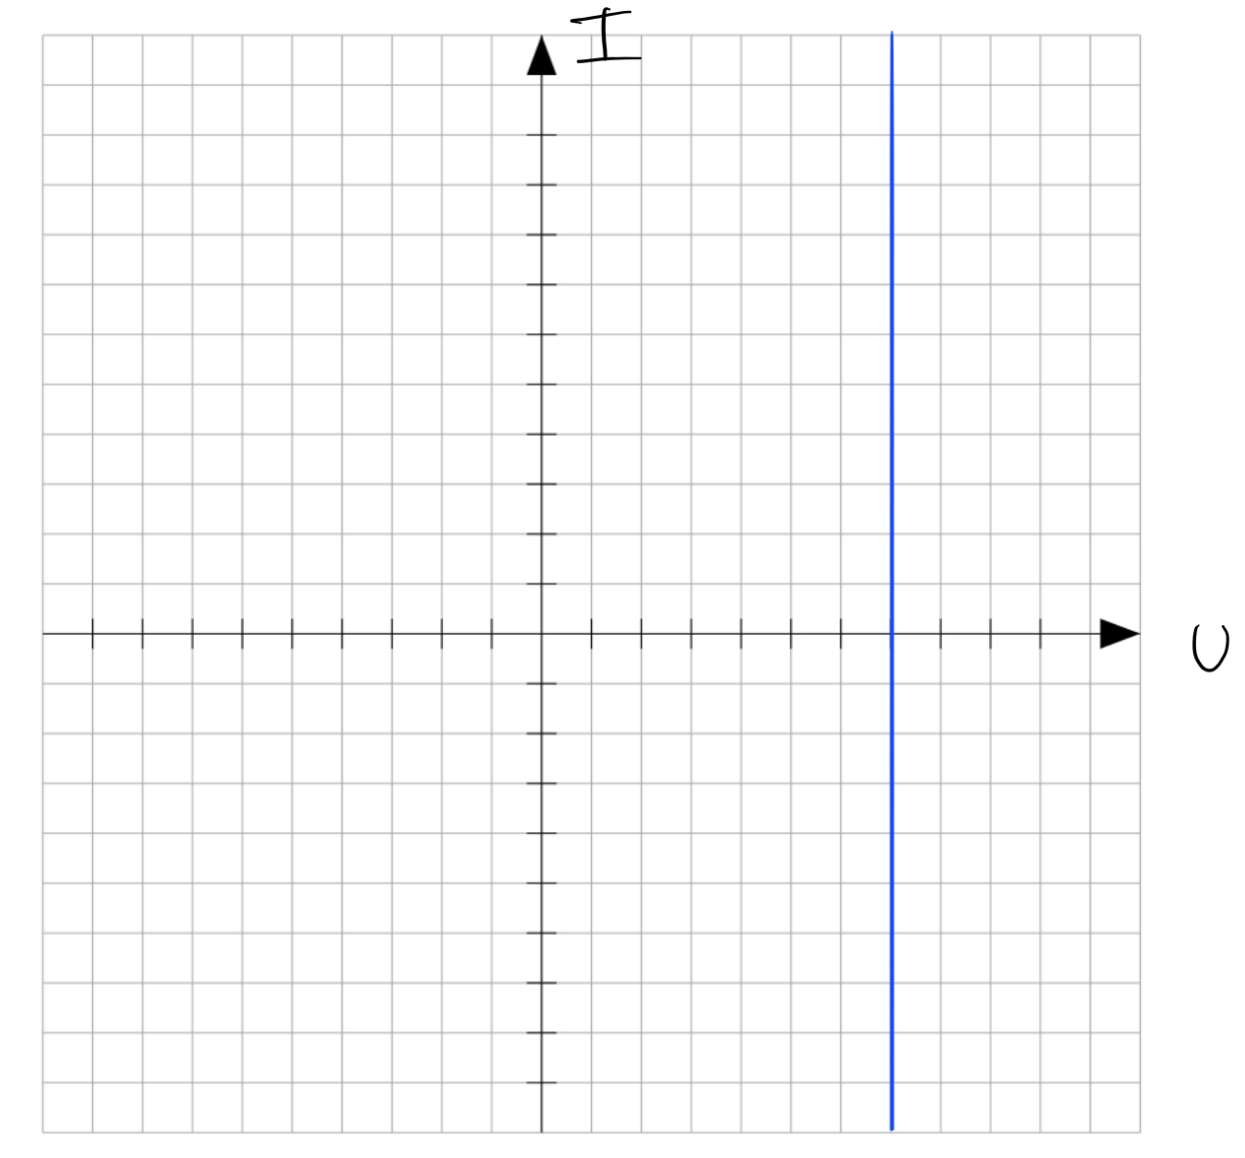
\includegraphics[width=\textwidth]{Voraufgaben/Ce.jpg}
        \caption{}
        \label{fig:VA_C_e}
    \end{subfigure}
    \hfill
    \begin{subfigure}[b]{0.45\textwidth}
        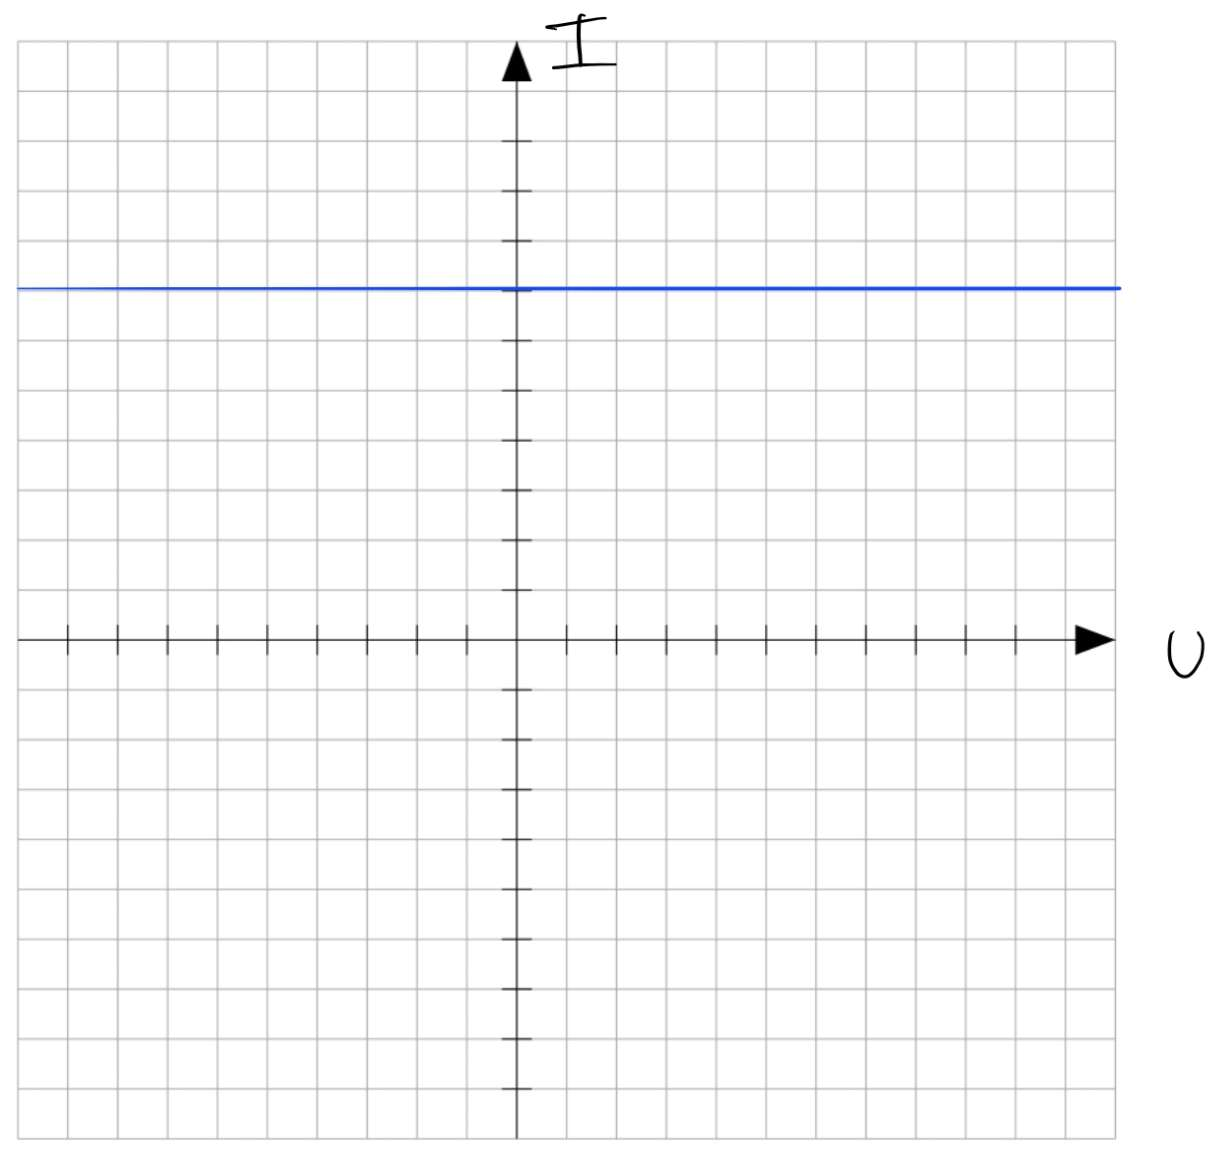
\includegraphics[width=\textwidth]{Voraufgaben/Cf.jpg}
        \caption{}
        \label{fig:VA_C_f}
    \end{subfigure}
    \caption{Kennlinienverläufe einiger Zweipole}
\end{figure}



% Text zu (c)
Zu c) : Reihenschaltung; der Gesamtstrom $I$ der Schaltung fließt durch Diode D und Widerstand $R$:

\[
I = \frac{U_D}{R_D} = \frac{U_R}{R} = \frac{U}{R + R_D}
\]

Die Kennlinie ist also fast wie bei der Diode, nur der Anstieg ab der Schwellenspannung ist kleiner.
\\

% Text zu (d)
Zu d) : Parallelschaltung; der Gesamtstrom $I$ setzt sich aus dem Strom durch die Diode $I_D$ und den Strom durch den Widerstand $I_R$ zusammen:

\[
I = I_D + I_R = \frac{U_D}{R_D} + \frac{U_R}{R}
\]

Die einzelnen Kennlinien von $R$ und $D$ werden also lediglich addiert.


\subsection*{Aufgabe D}
% Theo
\begin{figure}[H]
    \begin{subfigure}[b]{0.45\textwidth}
        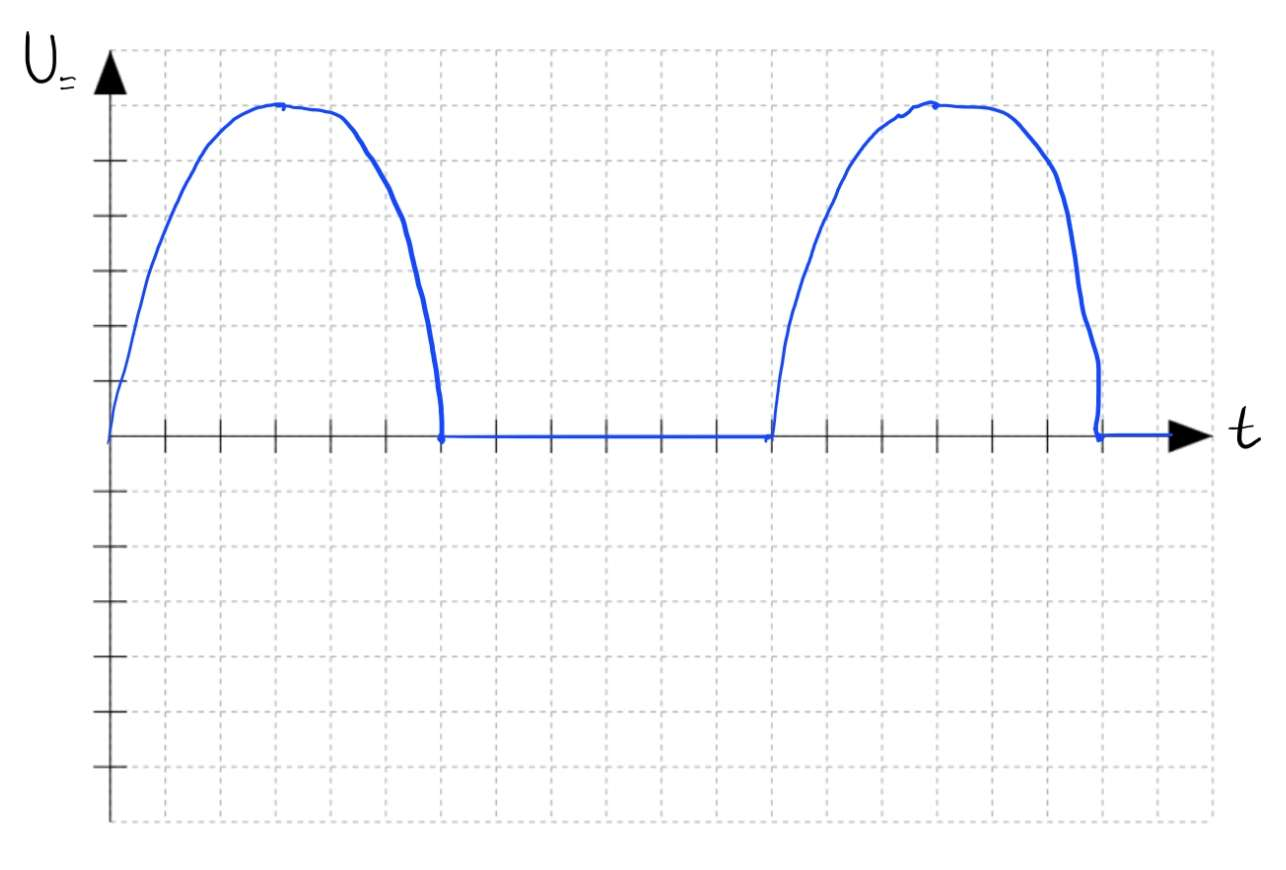
\includegraphics[width=\textwidth]{Voraufgaben/Da.jpg}
        \caption{}
        \label{fig:VA_D_a}
    \end{subfigure}
    \hfill
    \begin{subfigure}[b]{0.45\textwidth}
        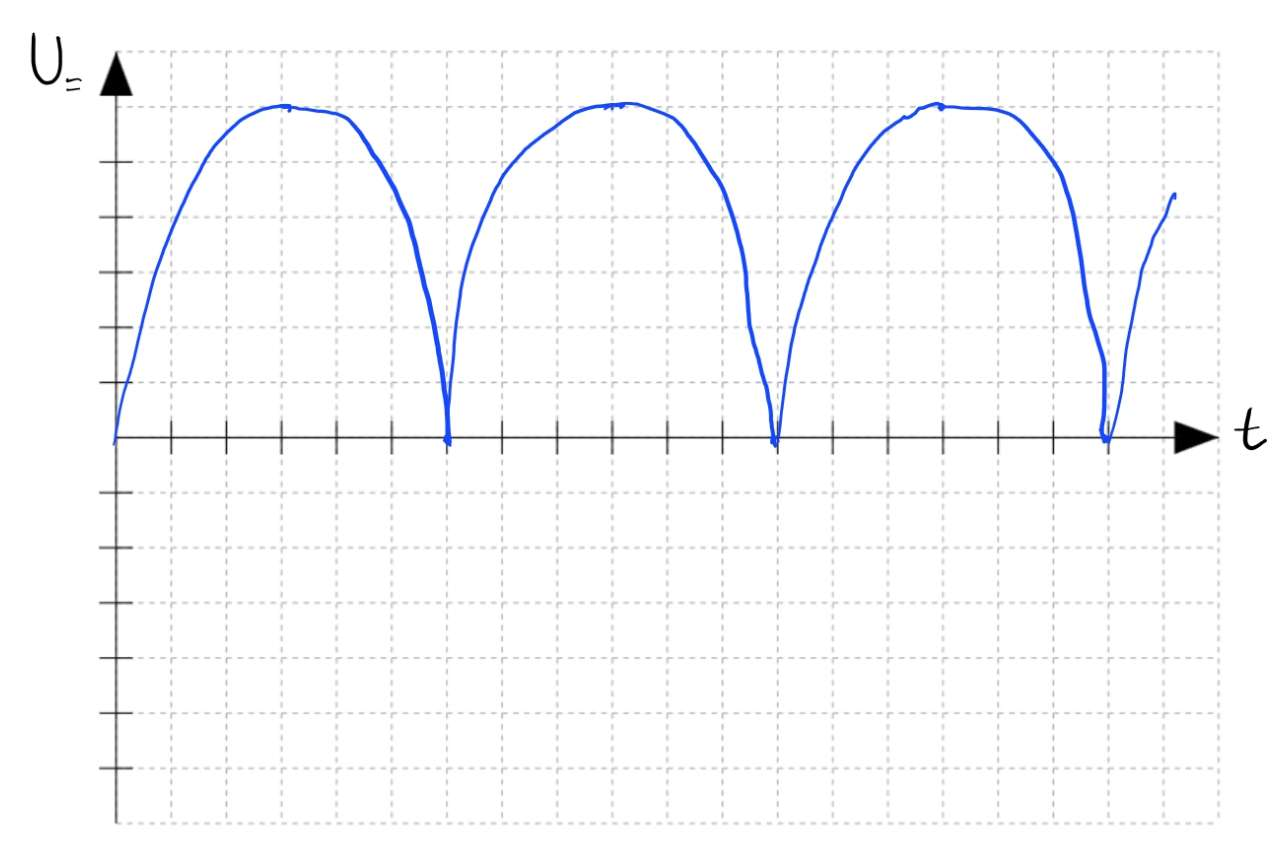
\includegraphics[width=\textwidth]{Voraufgaben/Db.jpg}
        \caption{}
        \label{fig:VA_D_b}
    \end{subfigure}
    \caption{Ein- und Zweiweggleichrichter}
\end{figure}

\subsection*{Aufgabe E}
\subsection*{Aufgabe F}
\subsection*{Aufgabe G}
\subsection*{Aufgabe H}
\subsection*{Aufgabe I}
% Theo
\begin{figure}[H]
    \begin{subfigure}[b]{0.45\textwidth}
        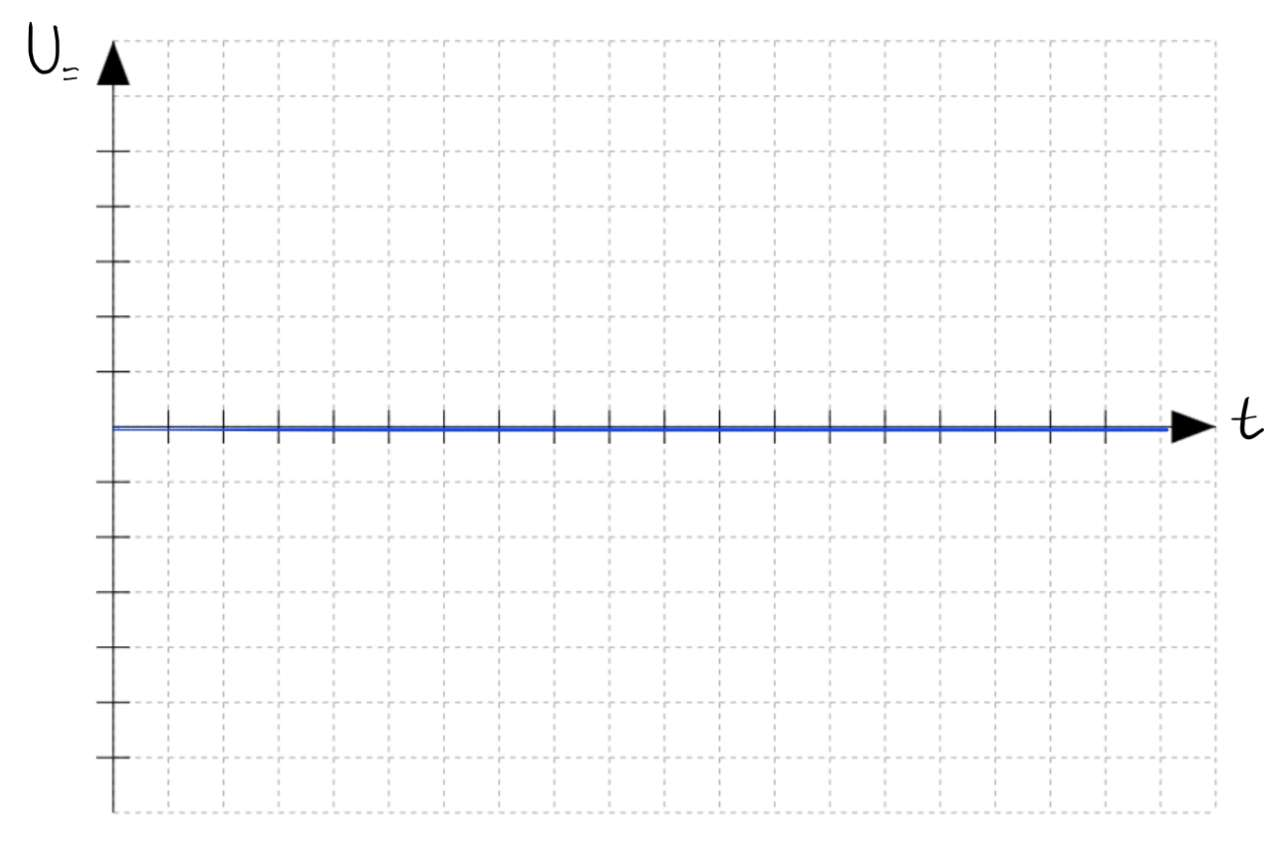
\includegraphics[width=\textwidth]{Voraufgaben/Ia.jpg}
        \caption{}
        \label{fig:VA_I_a}
    \end{subfigure}
    \hfill
    \begin{subfigure}[b]{0.45\textwidth}
        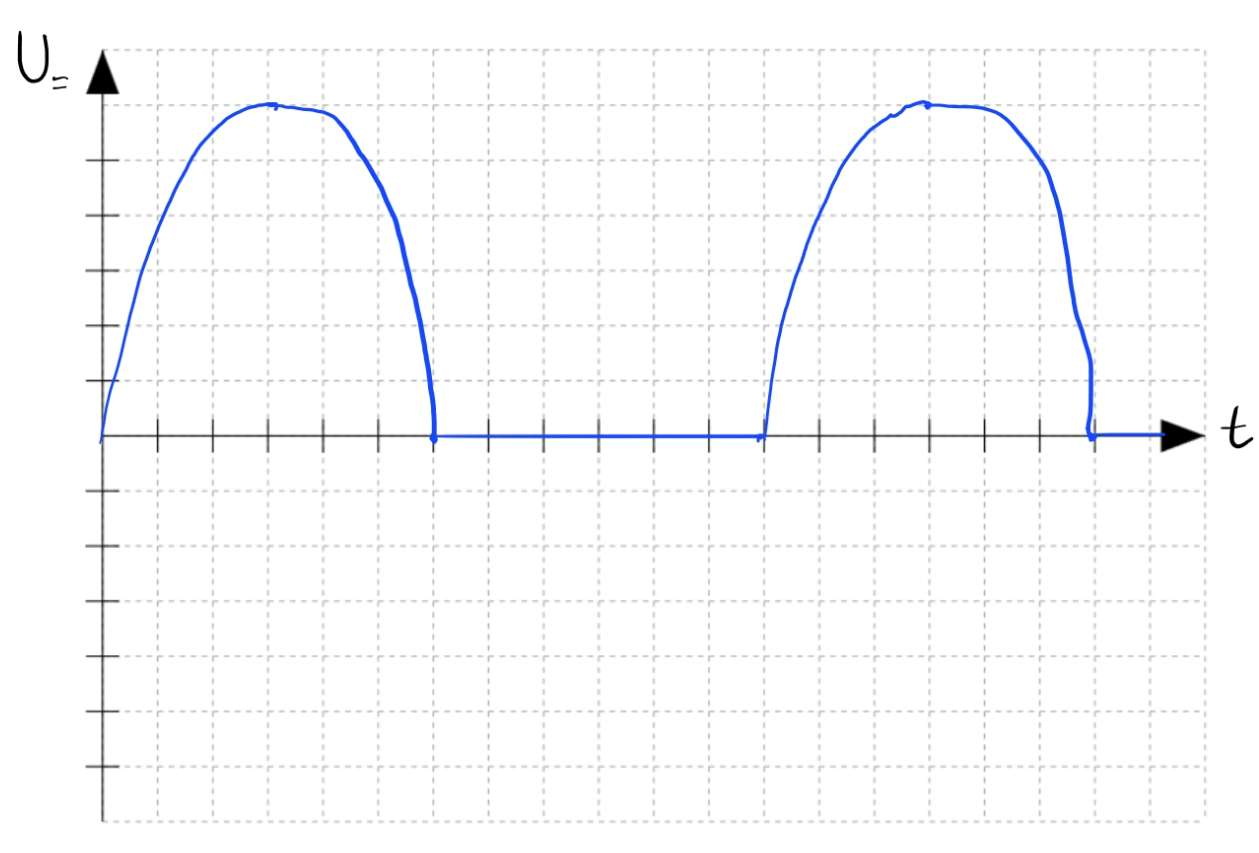
\includegraphics[width=\textwidth]{Voraufgaben/Ib,c.jpg}
        \caption{, (c)}
        \label{fig:VA_I_d}
    \end{subfigure}
    \caption{Ein- und Zweiweggleichrichtung mit dem Dioden-Schaltbrett}
\end{figure}

\subsection*{Aufgabe J}
% Theo

\begin{figure}[H]
    \centering
    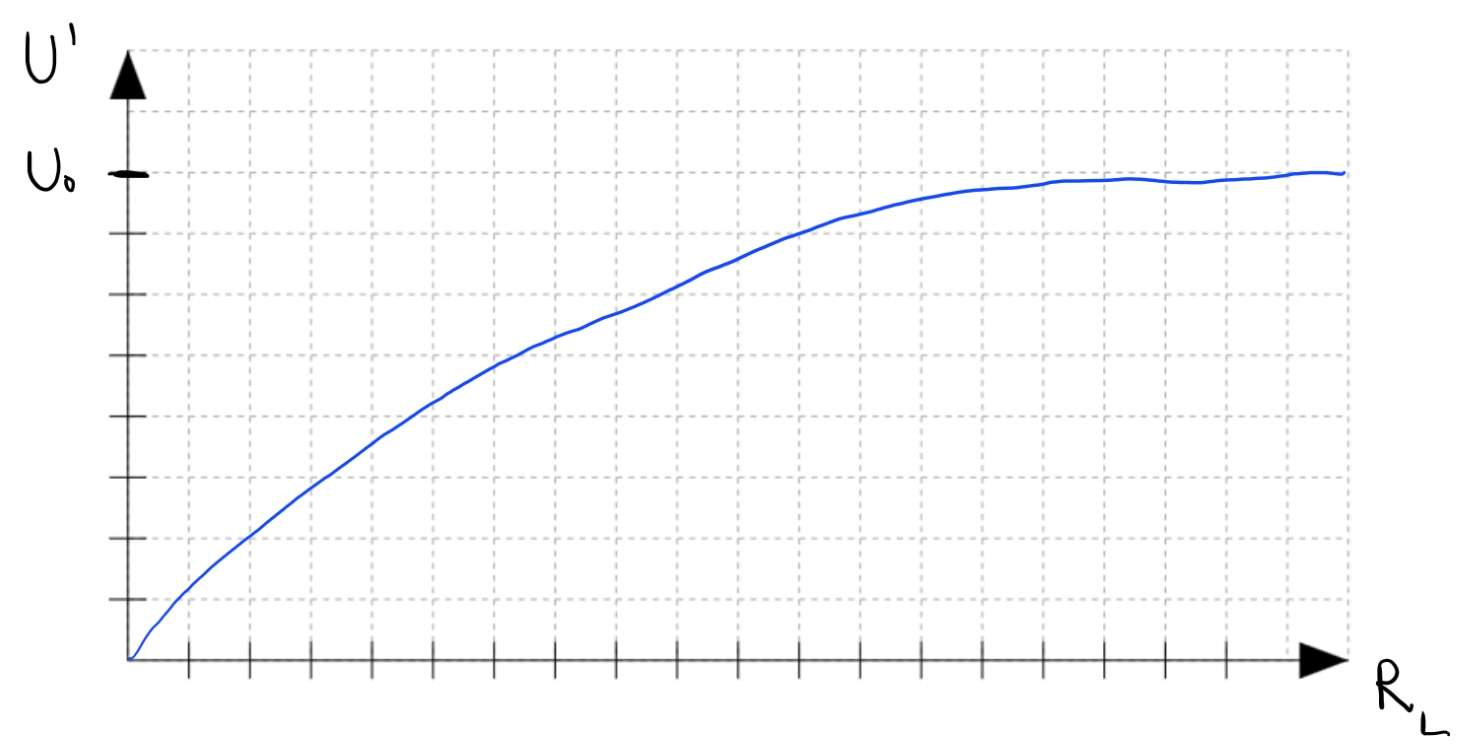
\includegraphics[width=0.7\textwidth]{Voraufgaben/J.jpg}
    \caption{Lastabhängigkeit der Spannung $U'$}
    \label{fig:VA_J}
\end{figure}

Es handelt sich um eine Spannungsteilerschaltung:

\[
U' = U_0 \cdot \frac{R_L}{R + R_L}
\]

Extremwerte:

\begin{itemize}
    \item $R_L \rightarrow 0 \Rightarrow U' \rightarrow 0$
    \item $R_L \rightarrow \infty \Rightarrow U' \rightarrow U_0$
\end{itemize}


\subsection*{Aufgabe K}